\documentclass[12pt, openany]{report}
\usepackage[utf8]{inputenc}
\usepackage[T1]{fontenc}
\usepackage[a4paper,left=2cm,right=2cm,top=2cm,bottom=2cm]{geometry}
\usepackage[frenchb]{babel}
\usepackage{libertine}
\usepackage[pdftex]{graphicx}
\usepackage{caption} 
\usepackage{float}
\usepackage{titlesec}
\usepackage{listings}
\usepackage[table,xcdraw]{xcolor}
\usepackage{bytefield}
\usepackage{verbatim}
\usepackage{hyperref}

\titleformat{\chapter}[display]{\normalfont\huge\bfseries}{}{20pt}{\Huge}

\setlength{\parindent}{1cm}
\setlength{\parskip}{1ex plus 0.5ex minus 0.2ex}
\newcommand{\hsp}{\hspace{20pt}}
\newcommand{\HRule}{\rule{\linewidth}{0.5mm}}

\begin{document}
\lstset{language=Java}
\begin{titlepage}
  \begin{sffamily}
  \begin{center}

    % Upper part of the page. The '~' is needed because \\
    % only works if a paragraph has started.
   % \includegraphics[scale=0.2]{logo_univ.jpg}~\\[1.5cm]

 	
    \textsc{\LARGE Université de Bordeaux}\\[3cm]

    \textsc{\Large Projet d'étude et de développement}\\[2.5cm]

    % Title
    \HRule \\[1.5cm]
    { \huge \bfseries Numérisation de façades par un essaim de drones\\[0.4cm] }

   % \HRule \\[2cm]
   % \includegraphics[scale=4]{logo_labri.jpg}
   % \\[2cm]
	
    \vspace{10 cm}
    
    % Author and supervisor
    \begin{minipage}{0.4\textwidth}
      \begin{flushleft} \large
      \emph{\textbf{Etudiants}}\\Guillaume Dupont\\Jérémy Poirier\\Alexandre Troncy
      \end{flushleft}
    \end{minipage}
    \begin{minipage}{0.4\textwidth}
      \begin{flushright} \large
        \emph{\textbf{Responsables}}\\Vincent Autefage\\Serge Chaumette\\Pascal Desbarats
      \end{flushright}
    \end{minipage}

    \vfill

    % Bottom of the page
    {\large Mars 2015}

  \end{center}
  \end{sffamily}
\end{titlepage}
%----------------------------------------------------------------------------------
\newpage
\tableofcontents
\begin{center}
\end{center}
%----------------------------------------------------------------------------------
\newpage
\chapter{Introduction au domaine}
Ce chapitre a pour objectif de cerner avec le moins d'ambiguïté possible le projet dans sa globalité ainsi que les différents comportements et services attendus par celui-ci. Nous définirons dans un premier temps le contexte du projet, puis nous ferons un état de l'art des projets existants ayant des problématiques proches.


\section{Introduction au projet}
La modélisation 3D est un domaine novateur aujourd'hui et de nombreuses solutions sont à l'étude quant à l'automatisation de ce procédé. Le projet consiste ici à numériser en 3D la façade d'un bâtiment en utilisant les caméras 2D de plusieurs drones de manière simultanée, et ce en utilisant le principe de la photogrammétrie. L'objectif est de reconstituer le nuage de points correspondant à la surface de la façade.
Ce projet sera mené en collaboration par des étudiants ayant des spécialités différentes, à savoir les domaines de l'image et celui des réseaux.

\subsubsection{Drone Bebop}

Le type de drone qui sera utilisé durant ce projet est le Parrot Bebop Drone. C'est un drone de loisir sorti en novembre 2014 dont les performances sont nettement supérieures à ses prédécesseurs (notamment en terme de stabilité de l'appareil, de la caméra ainsi que de la portée). On peut noter entre autres quelques caractéristiques : 
\begin{itemize}
\item Processeur double coeur Parrot P7
\item Processeur graphique quadri-coeur
\item Mémoire vive de 8 Go
\item Appareil photo "Fisheye" de 14 Mpx
\end{itemize}

\section{Etude de l'existant}
Nous présenterons dans cette partie les différents projets ayant des problématiques globales relativement proches du projet à effectuer. L'objectif est d'avoir une vue d'ensemble quant à ce qui existe déjà dans le domaine de la numérisation 3D effectuée à l'aide de drones.

\subsection{Projets existants utilisant les drones pour la modélisation}
Dans cette partie seront exposés les différents projets ou solutions d'entreprise relatant des problématiques proches du projet à réaliser.

\subsubsection{senseFly}
senseFly \footnote{\url{https://www.sensefly.com/home.html}} est une entreprise suisse filiale de Parrot proposant une solution de cartographie 2D et 3D à l'aide de drones autonomes. Ces cartographies permettent de récolter des informations utilisées notamment dans les domaines agricoles, miniers, humanitaires et de surveillance.

L'utilisateur définit dans un premier temps le plan de vol du drone à l'aide d'une application eMotion prenant en compte la topographie de la zone de vol et la force des vents. Ensuite, l'utilisateur lance simplement le drone qui suit son plan de vol et récupère des photos lors de son parcours. Enfin, une fois les photos récupérées, celles-ci peuvent être traitées via un logiciel de rendu 3D, PostFlight-Terra3D, ou tout autre logiciel de processus métier. Quelques caractéristiques de la solution :
\begin{itemize}
\item Les drones utilisés sont de type avionique
\item Les drones ont une autonomie de 50 min
\item Les photos récoltées sont de type aériennes
\item Pas de gestion de flotte de drones
\end{itemize}

\subsubsection{Drone Aero Services}
En réponse à une demande d'une institution régionale, l'entreprise a eu pour mission de reconstituer un terrain nécessitant une mise à jour cartographique\footnote{\url{http://droneaeroservices.com/octobre-2014-photogrammetrie-et-reconstitution-3d-pour-drone-aero-services/}}. Le drone utilisé a balayé le site à l'aide d'un GPS centimétrique sur plusieurs hauteurs et plusieurs angles. Une fois les clichés pris, des points servant de référence ont été définis et ont constitué un nuage de points, et c'est grâce à celui-ci que la reconsitution 3D fut réalisée.

\subsubsection{Studio Fly}
Dans la même optique et en optant pour la même démarche de reconnaissance avec les drones, l'entreprise Studio Fly\footnote{\url{http://www.dronethermographie.fr/modelisation3d-drone-studiofly-technologie/}} propose des solutions pour la modélisation dans divers domaines tels que le BTP, la géologie ou l'archéologie.

\subsubsection{iDroneX}
L'entreprise iDroneX\footnote{\url{http://www.idronex.fr/modelisation-3d/}} propose également ce type de services dans des applications majeures comme les chantiers, monuments ou projets immobiliers.

\subsection{Projets existants utilisant la photogrammétrie}

\subsubsection{PhotoModeler}
PhotoModeler permet de créer des modèles 3D à partir de photos. Il est utilisé entre autres pour l'archéologie, l'architecture ou encore la biologie.

Dans un premier temps, l'utilisateur doit charger les photos d'un objet, prises depuis différents points de vue. Ensuite, il y a plusieurs constructions du nuage possibles :
\begin{itemize}
\item L'utilisateur entre manuellement les points communs entre les différentes photos
\item L'utilisateur a pris des photos avec peu de différences entre chaque angle de vue, ce qui permet au logiciel de reconnaitre la proximité de chaque photo
\item L'utilisateur a placé des marqueurs sur l'objet au moment de prendre la photo, ce qui permet ensuite une reconnaissance automatique de la position de l'objet par le logiciel
\end{itemize}
Une fois le nuage de points calculé (quelque soit la méthode utilisée), un modèle 3D peut être obtenu.

\begin{figure}[H]
  \center
  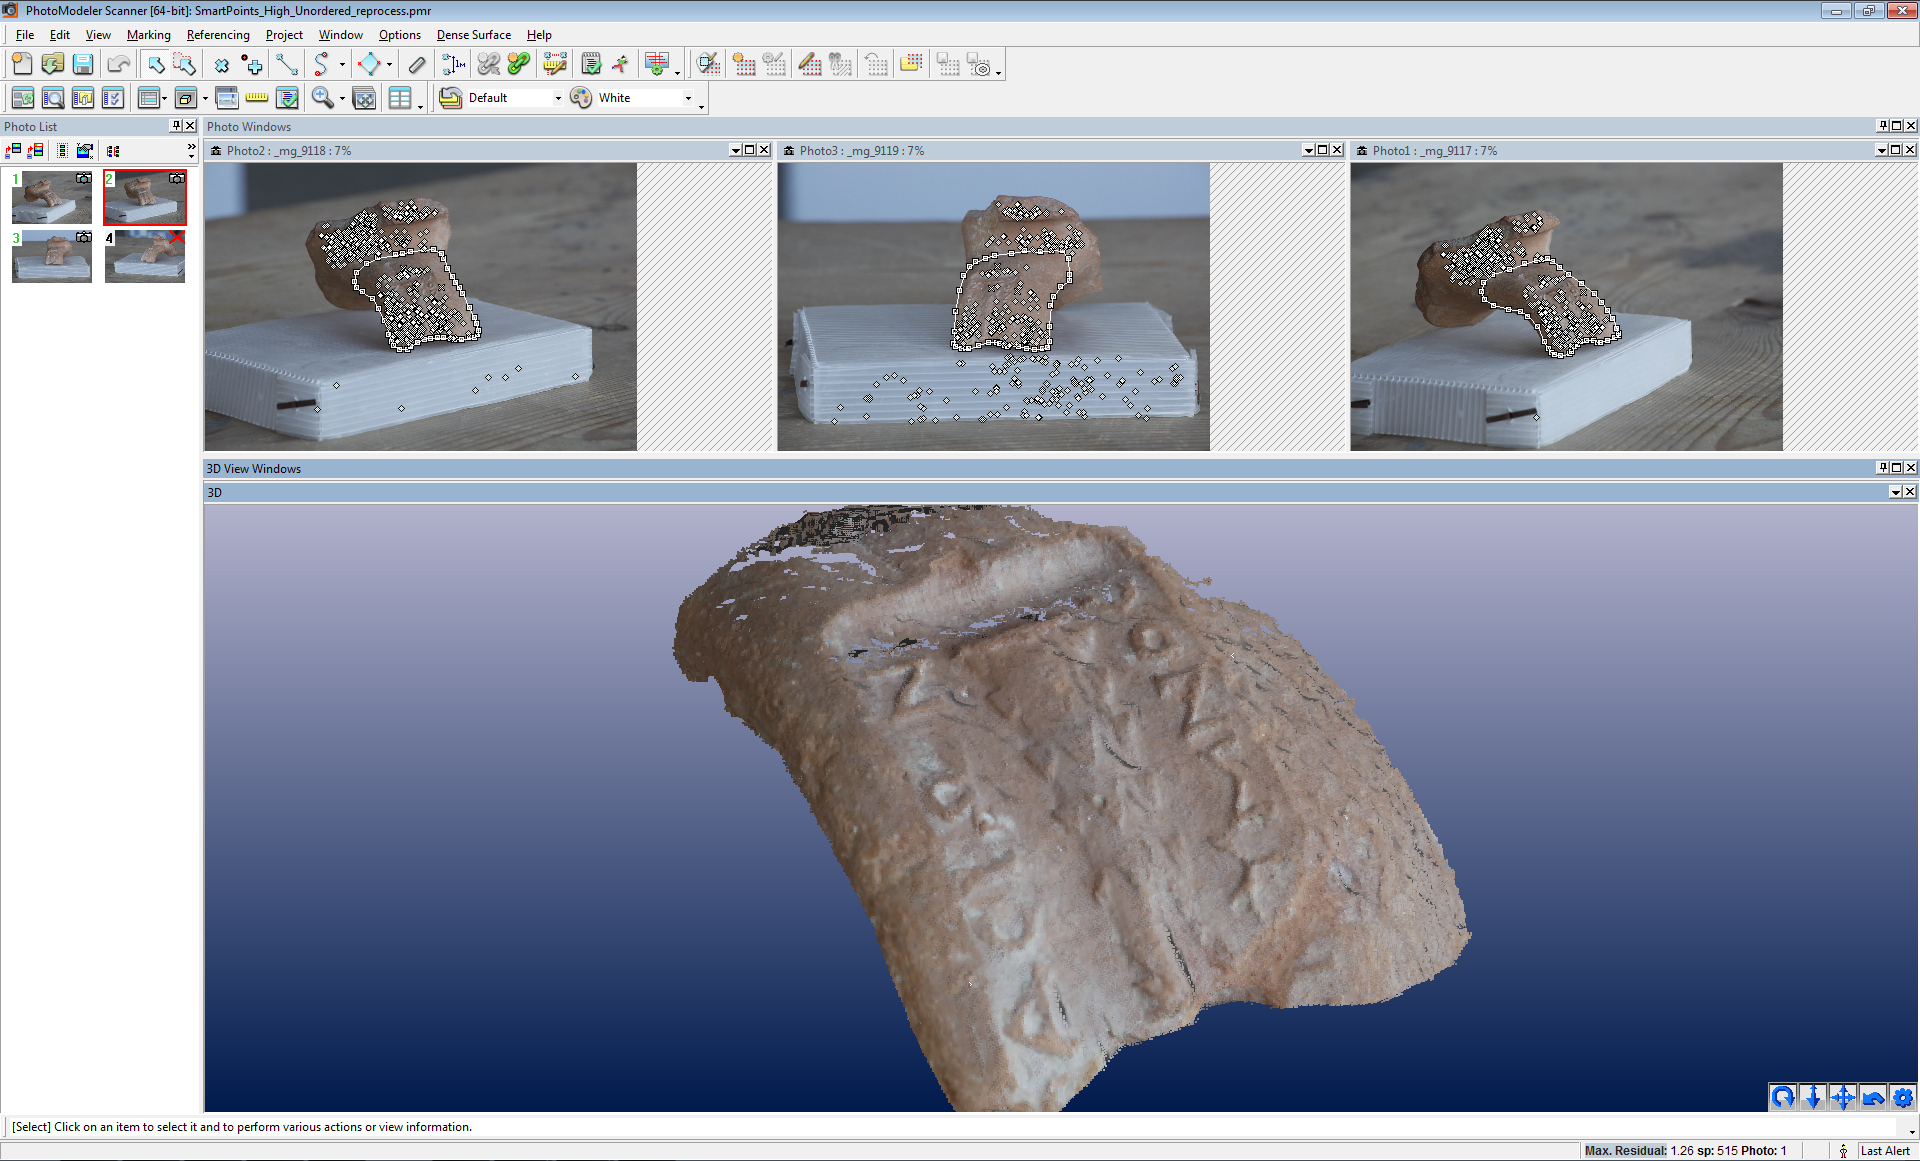
\includegraphics[scale=0.2]{figures/photomodeler.jpg}
  \caption{Capture d'écran du logiciel PhotoModeler}
  \label{fig:schema}
\end{figure}



\subsubsection{Free-D}
Free-D est un logiciel de reconstruction 3D.
Il offre les fonctionnalités suivantes :  
\begin{itemize}
\item Segmentation des images
\item Recalage des images
\item Reconstruction des surfaces
\item Affichage graphique des modèles
\end{itemize}

\begin{figure}[H]
  \center
  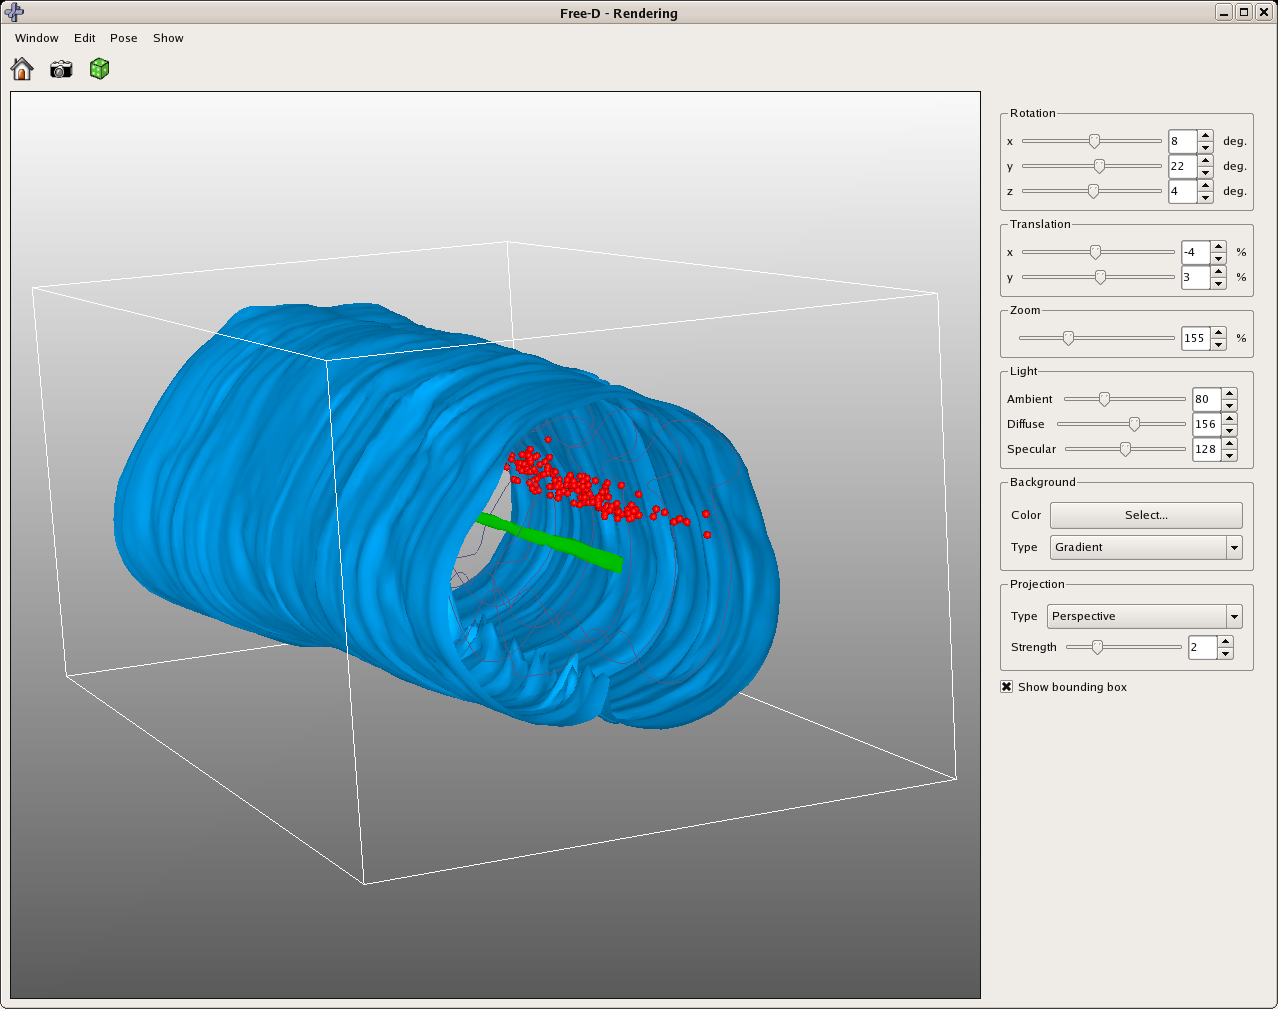
\includegraphics[scale=0.2]{figures/freeD.png}
  \caption{Capture d'écran du logiciel Free-D}
  \label{fig:schema}
\end{figure}

\chapter{Besoins}
Cette seconde partie est destinée à définir précisément les besoins de notre système. On distinguera parmi ces besoins les besoins fontionnels et non-fonctionnels de notre projet, définis dans les sections ci-dessous.

\section{Besoins fonctionnels}
Les besoins fonctionnels correspondent aux fonctionnalités attendues de
l’application. Ils précisent quels comportements et quels services le logiciel
devra fournir.

\begin{description}
\item[Supplanter l'OS du drone] \hfill \\
Dans un premier temps, il faudra installer un système d'exploitation sur une clé USB selon une certaine démarche et ensuite modifier la séquence de boot du drone de manière à supplanter le système du drone par un Linux sur-mesure. \\
\textit{\underline{Test} :} Après avoir effectué la manipulation, vérifier que le drone boot bien sur la clé et que le système fonctionne (comportement cohérent du drone).

\item[Retro-engineering] \hfill \\
Nous écouterons le trafic entre le drone et l’application pour smartphone FreeFlight3 (utilisée pour contrôler le drone). Nous récupérerons les paquets et les analyserons dans le but de retrouver les spécifications du protocole permettant de communiquer avec le Bebop. \\
\textit{\underline{Test} :} Effectuer une attaque MITM en utilisant \textit{arpspoof} et enregistrer les trames entre les deux parties, puis les analyser. Une fois le protocole identifié, tester l'envoi des commandes "forgées" au drone et vérifier son bon comportement.

\item[Pilotage des drones] \hfill \\
Les drones suivront un plan de vol en hauteur afin de recouvrir l'intégralité de la façade : ils devront se déplacer de bas en haut afin de recouvrir chacun une portion de la façade du bâtiment. Une interface graphique pourra être réalisée afin de faciliter le pilotage des drones et récupérer des informations en temps réel.\\
\textit{\underline{Test} :} Lancer le plan de vol sur plusieurs drones et constater leur bonne évolution dans l'espace en hauteur.

\item[Définir des points communs dans les vidéos] \hfill \\
Pour mener à bien la reconstitution par photogrammétrie, il est nécessaire que les vidéos prises par les drones durant leur vol aient des points en commun. Pour ce faire, une certaine distance entre eux sera définie. \\
\textit{\underline{Test} :} Lancer les deux vidéos et observer si elles contiennent des points similaires.

\item[Récupération de vidéo] \hfill \\
Il sera nécessaire de récupérer les vidéos prises par les drones et de la transmettre aux étudiants d'ISV afin de pouvoir réaliser par la suite la photogrammétrie. \\
\textit{\underline{Test} :} Récupérer sur le serveur \textit{ftp} du Bebop le fichier vidéo voulu, le transmettre et vérifier que l'envoi et la réception se sont déroulés correctement.


\end{description}


\section{Besoins non-fonctionnels}
Les besoins non-fonctionnels définissent des qualités générales qui ne sont pas liés directement aux services spécifiques délivrés par le système, mais qui définissent des aspects qui engendreront une meilleure utilisation de l'application. Ces éléments s'appliquent généralement au système dans son ensemble.


\begin{description} 
\item[Synchronisation entre les drones lors du recouvrement vidéo] \hfill \\
On pourra penser à définir des points d'attente lors du vol (ligne, laser, ...), pour qu'un drone en avance puisse attendre son semblable. Ainsi, une meilleure synchronisation permettra de faciliter le travail à effectuer pour la modélisation 3D car les deux vidéos auront les mêmes séquences d'images. \\
\textit{\underline{Test} :} Lancer le plan de vol sur plusieurs drones et constater leur évolution dans l'espace en hauteur synchronisée, selon la solution choisie.

\item[Convertir les vidéos] \hfill \\
Les étudiants d'ISV utilisent la bibliothèque OpenCV et de ce fait nécessitent un certain format vidéo pour réaliser la photogrammétrie, lisible par celui-ci. Le format le plus optimum est AVI car il est mieux géré sur les différentes plateformes existantes. On pensera donc à convertir le format MP4 par défaut des vidéos du Bebop en AVI. \\
\textit{\underline{Test} :} Récupérer en entrée un fichier présent sur le Bebop au format MP4 en ayant pris soin de vérifier que la vidéo se lit correctement, et vérifier en sortie que le fichier obtenu est au format AVI et lisible également.

\item[Récupération d'informations] \hfill \\
Nous pourrons penser à récupérer des informations lors du vol des drones au travers d'une interface graphique dans le but de suivre leurs évolutions respectives pendant le vol.\\
\textit{\underline{Test} :} Vérifier le bon affichage en temps réel des informations sur l'interface graphique.
\end{description}

\chapter{Spécificités du Parrot Bebop}
Le but de ce chapitre est de rendre compte des différences et nouveautés apportées par le Parrot Bebop. Nous y détaillerons la démarche suivie pour la supplantation d'un Linux sur-mesure sur le drone, ainsi que les spécifications du nouveau protocole utilisé pour le piloter.

\section{Particularités}
Dans cette partie seront exposés des faits divers sur le Bebop constituant des informations à prendre en compte lors d'un travail à effectuer avec un tel drone. Parmi les informations pertinentes à retenir, on peut relever que : 
\begin{itemize}
\item L'adresse IP par défaut du drone est \textit{192.168.42.1}.
\item Le drone dispose d'un serveur \textit{ftp} sur lequel on peut se connecter sans avoir besoin de mentionner des informations de connexion. Ce serveur donne accès aux fichiers à partir de \textit{/data/ftp}.
\item Le drone et le contrôleur interagissent par défaut via deux ports : 
\begin{lstlisting}[frame=single]
c2dport: 54321
d2cport: 43210
\end{lstlisting}
\item Il est possible de se connecter en réseau avec le drone en le connectant depuis son port USB. Dans ce cas, son adresse par défaut devient \textit{192.168.43.1} et pour ce faire il faut exécuter le script :
\begin{lstlisting}[frame=single]
/ # /bin/usbnetwork.sh
\end{lstlisting}
\item Le démon \textit{dragon-prog} est lancé au démarrage et gère le système.
\item Pour lancer le mode \textit{Debug}, il faut exécuter le script :
\begin{lstlisting}[frame=single]
/usr/bin/DragonDebug.sh
\end{lstlisting}
\item Un SDK\footnote{\ url{https://github.com/ARDroneSDK3}} a été mis en place pour le Parrot Bebop.
\end{itemize}

\section{BebopXT}
Le système d'exploitation du drone étant propriétaire et une mauvaise manipulation étant rédhibitoire, la mise en place d'un autre système pour supplanter ce dernier semble pertinent. Ce dernier sera pré-installé sur une clé USB. 
La démarche générale afin de mettre en place un tel système est principalement la même que pour l'ArDroneXT \footnote{\url{http://hal.archives-ouvertes.fr/hal-00916815}}. Néanmoins, quelques différences sont à noter :
\begin{itemize}
\item Le système du drone ne reconnaît pas le format \textit{ext2}. De ce fait, lors de l'installation des 3 partitions sur la clé USB, il faut désormais formater le système de fichiers des partitions ARDSYS et ARDDEV en \textit{ext3}.
\item Contrairement à l'ArDrone2, le debootstrap n'a pas fonctionné en utilisant le système d'exploitation \textit{Squeeze}, ce à quoi nous avons solutionné le problème en utilisant la version plus récente \textit{Wheezy}.
\item Lors de la manipulation délicate de création du script d'initialisation qui monte la partition ARDSYS (\textit{xtStart}), et de l'appel à celui-ci dans le processus qui initialise le drone (\textit{rcS}), la ligne de code suivante ne devra plus être intégrée dans le script directement (avec la commande \textit{echo}) mais ajoutée à la fin du fichier : 
\begin{lstlisting}[frame=single]
# Ligne a ne plus inclure dans le script mais a ajouter 
# manuellement dans le fichier rcS
echo '/etc/init.d/xtStart &' >> /etc/init.d/rcS  
\end{lstlisting}
\end{itemize}

\section{Initialisation de la communication}
Pour initialiser la communication avec le Bebop, il est nécessaire d'envoyer à ce dernier un message au format JSON sur le port TCP 4444.
La requête JSON prend la forme suivante :
\begin{verbatim}
{"controller_name":"toto","controller_type":"toto","d2c_port":43210}
\end{verbatim}
Celle-ci détermine un nom, un type de contrôleur et le port que le drone utilisera pour communiquer avec le contrôleur. Pour maintenir la communication, il est nécessaire que le contrôleur envoie un message régulièrement au drone ; dans le cas contraire, ce dernier coupe la communication. Dans la section suivante, nous analyserons le protocole nécessaire pour communiquer avec le drone. 

\section{Protocole ArDrone 3}
Parrot a mis en place un protocole dédié à la communication entre ses derniers drones (Bebop, Jumping Sumo et Rolling Spider), et son contrôleur. Il est intéressant de noter que le protocole utilise l'endianisme \textit{little endian}, alors que le \textit{big endian} est majoritairement utilisé pour les protocoles de transmission. Dans cette partie, nous expliquerons le principe de fonctionnement du protocole.
\subsection{En-tête}

\begin{figure}[!h]
\begin{center}
\begin{bytefield}[bitwidth=0.6em]{56}
\bitheader{0,7,8,15,16,23,24,55} \\
\bitbox{8}{type} & \bitbox{8}{id} & \bitbox{8}{seq} & \bitbox{32}{size} \\
\end{bytefield}
\end{center}
\caption{En-tête Protocole Ar Drone 3}
\end{figure}

Tous les messages de communication entre le drone et le contrôleur utilisent la même en-tête. Celle-ci est codée sur 7 octets, contenant les champs \textit{type}, \textit{id} , \textit{seq} et \textit{size} que nous décrirons ci-après.

\begin{itemize}
\item \textit{Type} : Ce champ, codé sur un octet, détermine le type du message. Celui-ci peut valoir quatre valeurs différentes, détaillées ci-dessous :
	\begin{enumerate}
	\item Message d'acquittement
    \item Message d'envoi de données
    \item Message à faible latence
    \item Message d'envoi de données qui requiert un acquittement
	\end{enumerate}
\item \textit{Id} : ce champ, codé sur un octet, détermine le buffer employé pour le message, celui-ci est compris entre 10 et 127 selon le SDK. Néanmoins ce champ subit des modifications en fonction du type de message et de l'émetteur (contrôleur ou drone), sa valeur réelle est comprise entre 10 et 254. 
\item \textit{Seq} : ce champ, codé sur un octet, détermine le numéro de séquence d'un message. Il existe plusieurs numéros de séquence dans le protocole, un par type.
\item \textit{Size} : ce champ, codé sur 4 octets, détermine la taille complète du message et non la taille du datagramme.
\end{itemize}

Dans la suite nous présentons la structure des paquets en fonction de leur type.

\subsection{Message d'envoi de données avec ou sans acquittement}

\begin{figure}[!h]
\begin{center}
\begin{bytefield}[bitwidth=0.55em]{64}
\bitheader{0,7,8,15,16,23,24,55,56,63} \\
\bitbox{8}{type} & \bitbox{8}{id} & \bitbox{8}{seq} & \bitbox{32}{size} & \bitbox{8}{project} \\
\bitbox{8}{class} & \bitbox{16}{cmd} & \bitbox{40}{*args (size-11)}
\end{bytefield}
\end{center}
\caption{Structure d'envoi de données avec un en-tête}
\end{figure}

Les messages d'envoi de données avec ou sans acquittement (type 2 et 4) disposent de la même structure de message. Celle-ci est codée au minimum sur 4 octets, contenant les champs \textit{project}, \textit{class}, \textit{cmd} et occasionnellement \textit{args}, que nous décrirons à la suite.

\begin{itemize}
\item \textit{Project}: ce champ, codé sur un octet, détermine le projet auquel ce message est destiné. Il existe dans le SDK \footnote{\url{https://github.com/ARDroneSDK3/libARCommands/tree/master/Xml}} huit projets référencés, deux projets pour chaque drone et deux projets communs à l'ensemble des drones. On note cependant à travers nos captures qu'il existe d'autres projets, non référencés. Chaque projet a un identifiant unique représenté dans ce champ.
\item \textit{Class}: ce champ, codé sur un octet, détermine la classe d'un projet utilisé auquel ce message est destiné. Chaque classe a un identifiant unique représenté dans ce champ.
\item \textit{Cmd}: ce champ, codé sur 2 octets, détermine la commande d'une classe d'un projet utilisé auquel ce message est destiné. Une commande peut comprendre des arguments ou pas. Chaque commande a un identifiant unique déterminé par sa déclaration dans sa classe.
\item \textit{Args}: ce champ, codé sur la taille complète du message moins 11, détermine les arguments d'une commande. Un argument peut avoir de multiples types de données : entier non signé et signé sur 8 à 64 octets, des enumérations codés sur 4 octets, des flottants à simple précision et double précision codés selon la norme IEEE-754 ou des chaines de caractères.
\end{itemize}

\subsection{Message d'acquittement}
 
\begin{figure}[!h]
\begin{center}
\begin{bytefield}[bitwidth=0.55em]{64}
\bitheader{0,7,8,15,16,23,24,55,56,63} \\
\bitbox{8}{type} & \bitbox{8}{id} & \bitbox{8}{seq} & \bitbox{32}{size} & \bitbox{8}{ack} \\
\end{bytefield}
\end{center}
\caption{Structure d'un acquittement avec un en-tête}
\end{figure}

Les messages d'acquittement font suite à des messages d'envoi avec acquittement (type DATA\_WITH-ACK). L'unique champ de ce message, codé sur un octet, correspond au numéro de séquence du message à acquitter.


\subsection{Message à faible latence}

Les messages à faible latence sont principalemement utilisés pour la transmission du flux vidéo. Ces messages disposent de deux structures : une structure d'envoi du flux vidéo du drone au contrôleur et une structure d'acquittement du flux vidéo du contrôleur au drone. 

\begin{figure}[!h]
\begin{center}
\begin{bytefield}[bitwidth=0.6em]{56}
\bitheader{0,7,8,15,16,23,24,55} \\
\bitbox{8}{type} & \bitbox{8}{id} & \bitbox{8}{seq} & \bitbox{32}{size}\\
\bitbox{16}{frameNum} & \bitbox{8}{frameFlags} & \bitbox{8}{fragNum} & \bitbox{8}{fragFrame} & \bitbox[lrt]{16}{}\\
\wordbox[lrb]{1}{*data (size-12) (max 1000)}
\end{bytefield}
\end{center}
\caption{Structure d'envoi du flux vidéo}
\end{figure}

La structure des messages d'envoi de flux vidéo est codée au minimum sur 6 octets. Celle-ci contient les champs \textit{frameNumber}, \textit{frameFlags}, \textit{fragmentsNumber}, \textit{fragmentsPerFrame} et \textit{data}.

\begin{itemize}
\item \textit{frameNumber} : ce champ, codé sur 2 octets, détermine le numéro de la trame vidéo.
\item \textit{frameFlags} : ce champ, codé sur un octet, détermine le flag de la trame. Nous n'avons cependant pas trouvé à quoi correspond chaque flag.
\item \textit{fragmentNumber} : ce champ, codé sur un octet, détermine le numéro de fragment d'une trame vidéo.
\item \textit{fragmentsPerFrame} : ce champ, codé sur un octet, détermine le nombre de fragments pour une trame vidéo. Une trame peut être fragmentée au maximum 128 fois.
\item \textit{data} : ce champ, codé sur la taille complète du message moins 12, détermine les données du flux vidéo. Le champ de données a pour taille maximale 1000 octets.
\end{itemize}


\begin{figure}[!h]
\begin{center}
\begin{bytefield}[bitwidth=0.6em]{56}
\bitheader{0,7,8,15,16,23,24,55} \\
\bitbox{8}{type} & \bitbox{8}{id} & \bitbox{8}{seq} & \bitbox{32}{size}\\
\bitbox{16}{frameNum} & \bitbox[lrt]{40}{highPacketAck} \\
\bitbox[lrb]{24}{} &\bitbox[lt]{8}{} &\bitbox[rtb]{24}{lowPacketAck} \\
\bitbox[lrb]{32}{}
\end{bytefield}
\end{center}
\caption{Structure d'acquittement du flux vidéo}
\end{figure}

La structure des messages d'acquittement de flux vidéo est codée sur 131 octets. Celle-ci contient les champs \textit{frameNumber}, \textit{highPacketAck} et \textit{lowPacketAck}.Les champs \textit{highPacketAck} et \textit{lowPacketAck} déterminent l'état d'avancement de l'acquittement d'une trame. Chaque bits de ces deux champs représentent un fragment d'une trame acquitté avec la valeur 1 ou non acquitté avec la valeur 0. Sachant qu'une trame ne contient pas toujours 128 fragments, une fonction utilisant le poids de Hamming est mise en place pour acquitter les fragments par défaut non compris dans la trame.

\begin{itemize}
\item \textit{frameNumber} : ce champ, codé sur 2 octets, détermine le numéro de la trame vidéo.
\item \textit{highPacketAck} : ce champ, codé sur 64 otctets, détermine l'acquittement des fragments 64 à 127.
\item \textit{lowPacketAck} : ce champ, codé sur 64 otctets, détermine l'acquittement des fragments 0 à 63.
\end{itemize}

\subsection{Concaténation de message}
Nous avons vu précédemment que le champ \textit{size} de l'en-tête déterminait la taille d'un message et non celle du datagramme. Dès lors, il est possible pour le protocole ArDrone3 de concaténer plusieurs messages dans un même paquet.

\subsection{Plugins Wireshark}

Au cours du projet, nous avons effectué de nombreuses captures de paquets pour comprendre le fonctionnement du protcole ArDrone3. Pour mieux analyser ces captures, nous avons également codé un plugin minimaliste pour le logiciel Wireshark. Celui-ci met en avant la plupart des champs mentionnés auparavant.


\begin{figure}[!h]
  \centering
  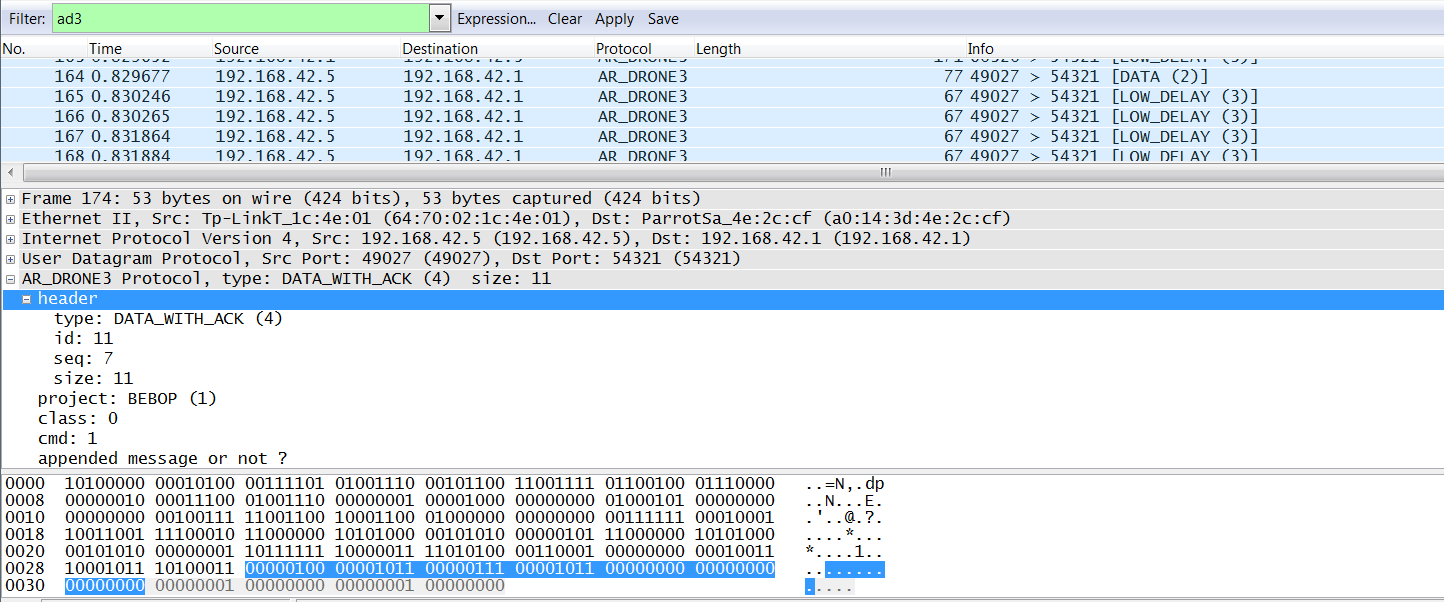
\includegraphics[width=\textwidth]{figures/dis.png}
  \caption{Capture d'écran plugins Wireshark ArDrone3}
  \label{fig:schema}
\end{figure}

\chapter{Scénario d'utilisation}

Nous présenterons ici un scénario d'utilisation de notre projet en trois phase (voir Fig. 4.1).

\section{Initilisation}

Dans un premier temps l'utilisateur lance notre programme. Ce dernier établit la connexion avec les deux drones, puis met à disposition de l'utilisateur une interface. A partir de cette interface l'utilisateur peut appréhender les informations de navigations recu et émis par chaque drone. Il peut également insérer des paramêtres nécessaires à la numérisation de la façade : l'altitude maximal, la vitesse verticale et l'angle panoramique. Une fois les paramêtres rentré, il peut lancer la procédure de numérisation en appuyant sur le bouton Launch et l'arréter en cas de problème via la bouton Stop.

\section{Numérisation de la façade}

On considère que l'utilisateur à préalablement placé les deux drones face à la façade à numériser.

\begin{itemize}
\item \textit{En A} : Les deux drones sont aux sols convenablement placé par l'utilisateur.
\item \textit{De A à B} : Les deux drones entament leur décollage.
\item \textit{En B} : Une fois en vol stationnaire, les paramêtres de l'utilisateur sont envoyés et vérifiés. Puis on lance l'enregistrement vidéo. 
\item \textit{De B à C} : Les deux drones entament leur ascencions jusqu'à l'altitude maximale.
\item \textit{En C} : On stop l'enregistrement, et enfin ordonne l'ordre d'aterissage.
\end{itemize}



\section{Récupération et traitement de la vidéo}

L'Utilisateur peut finalement utiliser le bouton Vidéo de l'interface pour récupérer le dernier enregistrement qui sera convertie du format mp4 au format avi, utilisable par le programme du groupe d'ISV.

\begin{figure}[!h]
  \centering
  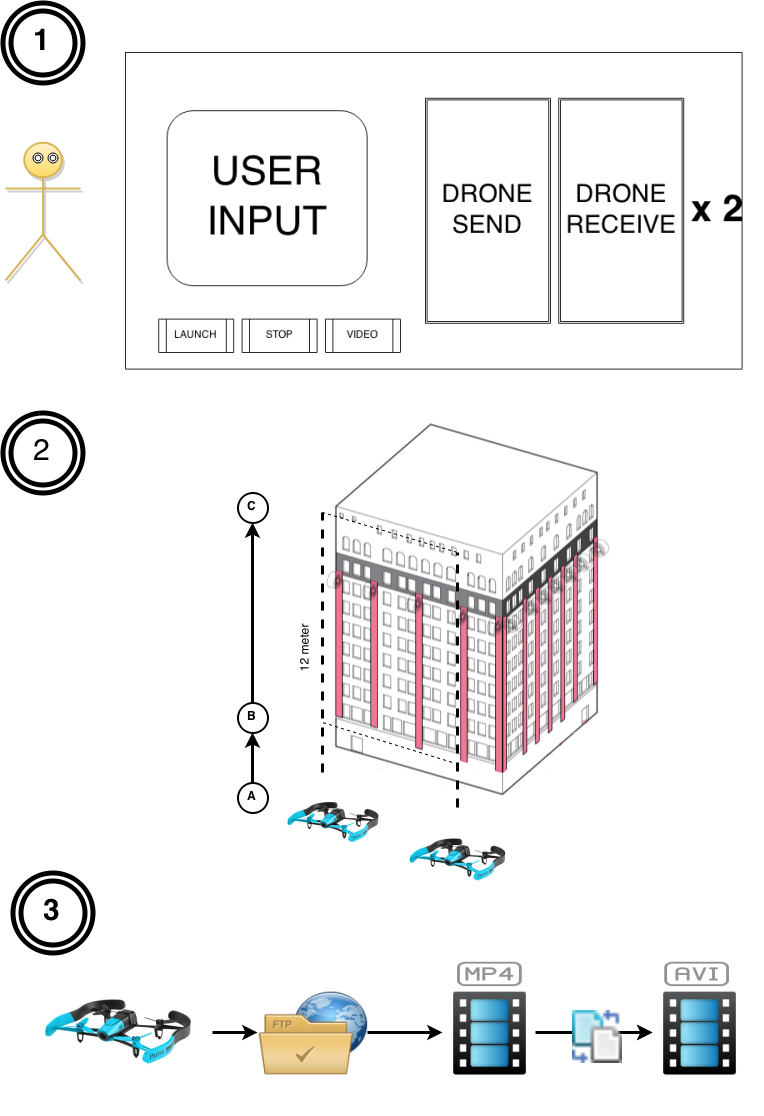
\includegraphics[width=\textwidth]{figures/osef.png}
  \caption{Phase d'utilisation}
  \label{fig:schema}
\end{figure}

\chapter{Architecture}

Nous présenterons ici le type d'architecture retenu dans le cadre de notre projet. 

\section{Modèle - Vue - Contrôleur}
Nous avons choisi d'utiliser un modèle MVC pour notre implémentation :

\begin{figure}[!h]
  \centering
  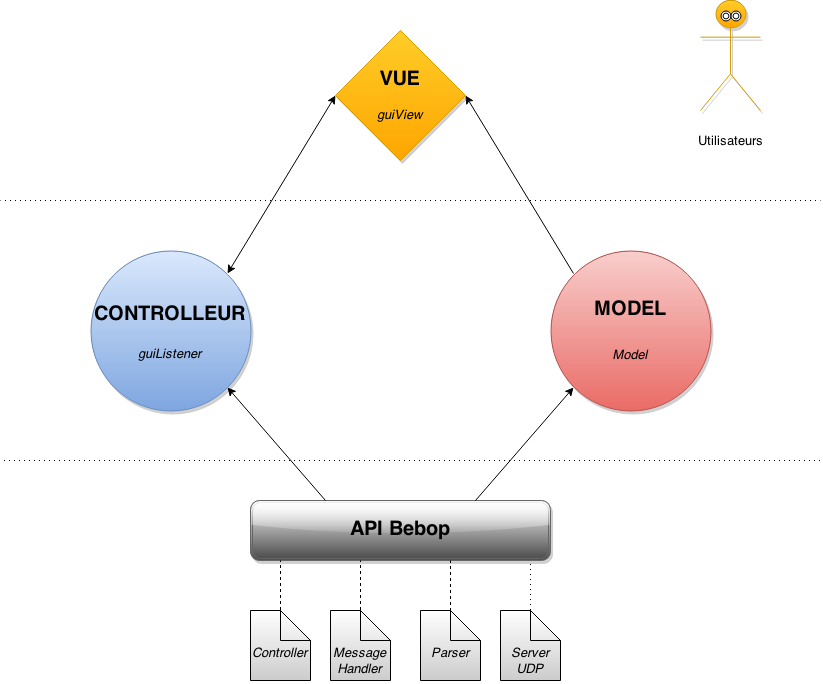
\includegraphics[width=\textwidth]{figures/ayylmao.png}
  \caption{Architecture MVC}
  \label{fig:schema}
\end{figure}
Les contrôleurs abritent la logique métier de l’application. Ils se chargent de traiter les données par l’utilisation du modèle adéquat et choisissent la vue à utiliser pour l’affichage.

Les vues correspondent à des parties d’IHM, elles sont dédiées à la présentation des informations. Aucun traitement de donnée n’est effectué dans une vue.

Les modèles gèrent l’accès aux données. Ils fournissent une abstraction en mettant à disposition des méthodes pour récupérer/insérer les informations sous une forme facilement manipulable par les contrôleurs et les vues.



\chapter{Résultats}
Nous présenterons dans cette partie les aboutissements de notre travail sur ce projet, en insistant particulièrement sur la réponse apportée aux différents besoins exposés précédemment.

\section{Commandes}
Lors de l'analyse des communications entre l'application FreeFlight 3 et le drone, nous avons pu observer la manière dont l'application envoie les commandes et ainsi reproduire ces commandes. A l'aide du SDK fourni par Parrot, nous avons pu forger en Java les commandes à envoyer pour interagir avec le drone et mener à bien sa mission. Comme nous souhaitions coder l'intégralité du projet en Java afin de pouvoir réutiliser quelques éléments développés lors de précédents projets (également en Java), il était plus simple pour nous de réécrire nos propres commandes, plutôt que d'utiliser le SDK tel quel.
Parmi toutes les commandes disponibles, nous nous sommes limités à celles qui nous sont utiles, entre autres:
\begin{description}
\item[setTime \& setDate] : Nécessaire pour l'enregistrement des vidéos.
\item[set max altitude \& speed] : Définit la vitesse maximale et l'altitude maximale.
\item[takeoff] : Permet de faire décoller le drone.
\item[landing] : Permet de faire attérir le drone.
\item[emergency] : Envoi un signal d'urgence au drone.
\item[gaz] : Permet de faire monter/descendre le drone.
\item[start \& stop recording] : Démarre/arrête l'enregistrement vidéo.
\end{description}

Pour forger une commande, on utilise l'objet \textit{Command} dont les attributs correspondent aux champs d'un message. Nous avons utilisé les champs suivants:
\begin{itemize}
\item byte \_type
\item byte \_id
\item byte \_seq
\item int \_size
\item byte \_project
\item byte \_class
\item short \_cmd;
\item byte[] \_arg;
\end{itemize}
On définit pour chacune des commandes les attributs ci-dessus avec les valeurs correspondantes trouvées dans le SDK. Par exemple, pour la commande \textbf{takeoff} :
\newpage
\begin{lstlisting}[frame=single]
public Command takeoff(byte seq){
	Command cmd_takeoff = new Command(TYPE_DATA_WITH_ACK,
		11, seq, BEBOP, PILOTING, TAKE_OFF);
	cmd_takeoff._size = 11;
	_cm.addText("take off");
	return cmd_takeoff;
}
\end{lstlisting}
Les différentes constantes sont définies afin de faciliter la création de commandes en concordance avec le SDK. On précise ensuite la taille du paquet : toutes les commandes ont une taille minimale de 11 octets. Finalement on utilise la variable \textit{\_cm} représentant une instance de \textit{ConsoleModel} afin d'afficher sur l'interface utilisateur un message explicitant la création et l'envoi du message (cf. 5.3)IHM). De plus, ce message est enregistré dans un fichier de log.

Avant d'envoyer une commande, on utilise la méthode \textbf{commandToByteArray()} qui convertit l'instance de \textit{Command} en un tableau d'octets qui sera envoyé \textit{via} le socket UDP. Chaque attribut de l'objet est ajouté à la bonne position dans le tableau en respectant les formats des paquets du protocole présenté plus haut. Dans le cas d'une commande prenant en argument une valeur de type \textit{float} ou \textit{double}, ces valeurs doivent être converties en IEEE-754. Prenons l'exemple de la méthode \textbf{doubleToIeee754(double value)}:
\begin{lstlisting}[frame=single]
public static byte[] doubleToIeee754 (double value){
	long holder = 0;
	holder = Double.doubleToRawLongBits(value);
	ByteBuffer buffer = ByteBuffer.allocate(Long.SIZE);
	buffer.order(ByteOrder.LITTLE_ENDIAN);
	buffer.putLong(holder);
	return buffer.array();
}
\end{lstlisting}
On appelle la méthode \textbf{doubleToRawLongBits(value)} afin de convertir la variable \textit{value} en IEEE-754 que l'on stocke dans une variable temporaire (\textit{long holder}). L'utilisation d'un \textit{long} permet de conserver le format IEEE-754. On utilise ensuite un \textit{ByteBuffer} en spéficiant l'ordre souhaité (\textit{little endian}) et l'on y insère la valeur de la variable \textit{holder}. Le tableau de d'octets retourné par la méthode sera ensuite ajouté aux arguments de la commande.


\section{Parser}
Lors de l'analyse des communications entre l'application FreeFlight 3 et le drone, nous avons pu obverser la manière dont le drone répond à l'application et ainsi comprendre son comportement. A l'aide du SDK fourni par Parrot, nous avons pu mettre en place en Java un \textit{parser} pour récupérer et analyser les données de navigation du drone afin de mener à bien sa mission. Parmi tous les messages "parsés", nous nous sommes limités à ceux qui nous sont utiles, à savoir :
\begin{description}
\item[getMaxAltitude \& getCurrentAltitude] : Permet de récupérer l'altitude maximale et l'altitude courante du drone.
\item[getMaxSpeed \& getCurrentSpeed] : Permet de récupérer la vitesse verticale maximale et la vitesse courante du drone.
\item[getDroneState] : Permet de récupérer le statut actuel du drone.
\item[getMediaRecordState] : Permet de récupérer le statut de l'enregistrement de la vidéo.
\end{description}

Pour \textit{parser} un message, on utilise l'objet \textit{Parser} dont les attributs correspondent aux champs d'un message. On parse les champs suivants:
\begin{itemize}
\item byte type
\item byte seq
\item int size
\item byte project
\item byte class
\item short cmd
\item ByteBuffer args
\end{itemize}

On définit dans un switch l'ensemble des \textit{type}, \textit{projet}, \textit{class} et \textit{cmd} nécessaires de "parser". Pour récupérer l'argument d'une commande, on utilise la valeur de \textit{size} et la taille constante d'une structure de message d'envoi de données. Par exemple pour le message \textit{getDroneState} : 
\begin{lstlisting}[frame=single]
case DATA:
project = packetAD3[offset+7]; 
switch(project){
  case PROJECT_BEBOP:
  classs = packetAD3[offset+8];
  cmd = packetAD3[offset+9];
  switch(classs){
    case CLASS_PILOTING_STATE:
	switch(cmd){
	  case CMD_FLYING_STATE_CHANGED:
	  args = ByteBuffer.wrap(packetAD3,offset+11,size-11);
	  _navData.setDroneState(args);
	  break;
\end{lstlisting}
Les différentes constantes sont définies afin de faciliter le "parsing" des messages. Les arguments \textit{size} et \textit{offset} nous permettent de "parser" les éventuels messages concaténés. De plus, lorsque nous recevons un message de type envoi avec acquittement, on se charge d'acquitter le message. Une fois l'argument récupéré, ce dernier est transmis à l'objet \textit{NavData} qui se charge de traiter l'information comprise dans l'argument afin d'afficher sur l'interface utilisateur les données de navigation actuelles du drone (cf. 5.3).

Certains arguments de commande, notamment l'altitude et la vitesse, retournent des données au format IEEE-754. Pour convertir ces données en valeurs pertinentes pour l'utilisateur, nous utilisons une fonction de conversion de ce type.

\begin{lstlisting}[frame=single]
private double ieee754ToDouble(ByteBuffer args){
	long holder = 0;
	args.order(ByteOrder.LITTLE_ENDIAN);
	holder = args.getLong();
	return Double.longBitsToDouble(holder);
}
\end{lstlisting}
L'utilisation d'un \textit{long holder} permet de contenir les 64 bits de données d'un flottant à double précisions sous le format IEEE-754. L'objet \textit{ByteBuffer} nous permet de préciser l'endianisme de la trame (\textit{little endian}) et de récupérer un \textit{long}. Enfin, la classe \textit{Double} se charge de convertir notre \textit{holder} en \textit{double}. Une fonction similaire existe pour les flottants.



\section{IHM}
L'interface homme-machine se présente de la sorte :

\begin{figure}[!h]
  \centering
  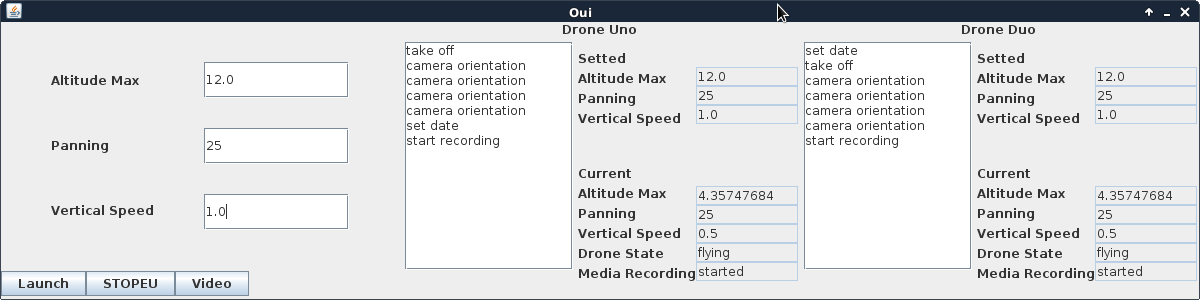
\includegraphics[width=\textwidth]{figures/ihm.png}
  \caption{Capture d'écran de l'IHM}
  \label{fig:schema}
\end{figure}
  
Après avoir exécuté le programme, l'utilisateur peut saisir trois informations en fonction de la façade à parcourir :
\begin{description}
\item[Altitude Max (m)] : L'altitude maximale du drone, typiquement la hauteur de la façade.
\item[Panning] : Le degré de la caméra sur le plan horizontal.
\item[Vertical Speed (m/s)] : La vitesse de montée du drone.
\end{description}
Comme expliqué précédemment, on retrouve les messages de \textit{log} dans les deux fenêtres à chaque envoi de commande. De plus, les deux drones nous renvoient en temps réel les informations relatives à leur vol (altitude, vitesse, en cours d'enregistrement ou non,...).
Enfin, le bouton \textbf{Launch} permet de démarrer la mission, le bouton \textbf{Stop} l'arrête, et le bouton \textbf{Video} démarre la récupération de la vidéo et sa conversion en AVI.


\section{Système de numérisation de façade automatisé}
L'utilisation de deux drones implique qu'ils soient tous deux synchronisés afin de fournir des vidéos exploitables. Une idée de synchronisme proposée avait été d'utiliser un laser. Toutefois, nous avons favorisé une approche plus naïve, en considérant leur vitesse de déplacement identique. Leur programme de vol se décompose en plusieurs phases :
\begin{description}
\item[Takeoff] Les deux drones décollent et attendent d'être tous deux dans le même état "hovering".
\item[Config] Configuration de la panoramique de la caméra, de l'altitude et vitesse maximum.
\item[MediaStarted] Démarrage de l'enregistrement.
\item[Flying] Phase de montée des drones, jusqu'à atteindre la hauteur saisie par l'utilisateur.
\item[MediaStopped] Arrêt de l'enregistrement.
\end{description}
Lors de chacune de ces phases, les \textit{threads} relatifs aux drones vont boucler après avoir effectuer chaque phase afin d'attendre si besoin que leur homologue termine sa phase en cours.


\section{Récupération de vidéo et conversion}
Dans le but de numériser la façade d'un bâtiment donné, les drones ont pour objectif de prendre des vidéos de la façade (une portion de bâtiment par drone). Une fois ces vidéos tournées, elles sont stockées directement dans la mémoire vive du drone. Ces vidéos sont par défaut enregistrées au format MP4, alors que le format attendu par nos collègues d'ISV est le format AVI (car mieux géré sur toutes les plateformes). L'objectif ici est donc d'automatiser la récupération et la conversion de ces vidéos. 


\subsection{Récupération de vidéo}
Le Bebop dispose d'un serveur FTP sur lequel nous pourrons récupérer ladite vidéo pour chaque drone :
\begin{lstlisting}[frame=single]
user@machine# ftp 192.168.42.1 21

#entrer un username
username : toto

# repertoire contenant les videos
ftp> cd internal_000/Bebop_Drone/media/	

# recuperation de la video voulue
ftp> get <nom_de_la_video>			

# suppression de la video pour desencombrer la memoire
ftp> delete <nom_de_la_video>				
\end{lstlisting}

Pour automatiser cette étape, nous avons utilisé le langage Python et plus particulièrement le module Pexpect afin de créer un processus fils simulant les commandes à effectuer pour récupérer la vidéo sur un drone. Ce script Python sera ensuite exécuté depuis l'interface graphique Java décrite précédemment.


\subsection{Conversion de vidéo}
La conversion du format MP4 en AVI s'effectue à l'aide de la solution FFMPEG, destinée au traitement de flux audio et vidéo. Le principe général de l'algorithme mis en place et de récupérer toutes les images de la vidéo à l'aide d'un objet de type \textit{FFmpegFrameGrabber} et de les enregistrer à l'aide d'un objet de type \textit{FFmpegFrameRecorder}. De fait, pour chaque image "saisie" par le grabber, nous l'enregistrons à l'aide du recorder au format désiré, en l'occurence le format AVI (format lisible par OpenCV).


\chapter{Difficultés rencontrées}
Ce chapitre est destiné à rendre compte des problèmes rencontrés lors du projet et qui ont gêné le bon déroulement de ce dernier.

\section{Mise à jour du firmware}
Plus ou moins régulièrement, Parrot déployait une mise à jour pour le Bebop, rendant impossible son utilisation avec notre OS "maison". Pour chaque nouvelle mise à jour, la manipulation fastidieuse suivante nous a ralenti :
\begin{enumerate}
\item Télécharger le fichier de mise à jour sur le site de Parrot
\item Le copier sur une clé USB formatée en FAT32
\item Brancher la clé sur le drone à l'aide d'un câble spécial (USB femelle, mini-USB mâle)
\item Démarrer le drone et attendre qu'il redémarre tout seul
\end{enumerate}
Cette manipulation a pour conséquence de réinitialiser le drone et ainsi d'effacer notamment notre script d'initialisation (\textit{xtstart}).


\section{Défaillance du drone}
Durant la dernière semaine de développement, nous avons rencontré un problème insolvable avec le drone : à chaque allumage du drone, son voyant d'état (normallement vert fixe) est rouge et clignote. En utilisant l'application FreeFlight 3 sur un smartphone OnePlus One, aucun problème n'est détecté : on peut se connecter au drone, on obtient bien le retour vidéo, on peut déplacer la caméra, toutefois il est impossible de le faire décoller. En utilisant l'application sur un Iphone, nous obtenons le message \textit{"Motor problem (1), go to motor settings for more information"}, bien qu'aucune erreur ne soit affichée sur la page dédiée aux moteurs. 
Après de nombreuses recherches et tentatives (hard reset, réinstallation du firmware), il semblerait qu'il faille le renvoyer au S.A.V.


\chapter{Conclusions et perspectives}
%conclusion
En définitive, ce projet de modélisation de façade en 3D à l'aide de drones nous a permis de travailler avec le nouveau drone Bebop et d'analyser ses différentes spécificités, notamment au niveau du nouveau protocole mis en place par Parrot. Notre application permet donc de contrôler le drone à l'aide des différentes commandes nécessaires pour le recouvrement vidéo de façades et de récupérer ces vidéos afin de les transmettre à nos collègues qui réalisent la photogrammétrie.

%perspectives
En guise d'améliorations, on pourrait penser à mettre en place un retour du flux vidéo de chaque drone en temps réel, pour que l'utilisateur soit assuré de sa prise vidéo. Il serait également intéressant de mettre en place un système permettant à l'utilisateur de traiter des façades nécessitant plusieurs prise de vue des drônes, en rajoutant de la synchronisation sur des mouvements latéraux. Voire calculer par un algorithme le nombre de traitements nécessaires en fonction de la superficie de la facade et la distance focale des drones. 

\end{document}